%
% Hello! Here's how this works:
%
% You edit the source code here on the left, and the preview on the
% right shows you the result within a few seconds.
%
% Bookmark this page and share the URL with your co-authors. They can
% edit at the same time!
%
% You can upload figures, bibliographies, custom classes and
% styles using the files menu.
%
% If you're new to LaTeX, the wikibook at
% http://en.wikibooks.org/wiki/LaTeX
% is a great place to start, and there are some examples in this
% document, too.
%
% Enjoy!
%
\documentclass[12pt,a4paper]{article}

\usepackage[german]{babel}
\usepackage[utf8x]{inputenc}
\usepackage{amsmath}
\usepackage{graphicx}


\title{Pflichtenheft VHDL}
\author{Arseniy Vershinin, Jonathan Kienzle, Amar Saljic}
\date{2 Mai, 2013}

\begin{document}
\maketitle

\section{Aufgabenverteilung}

{\bf Projektleiter:} Arseniy Vershinin\newline
{\bf Verantwortlicher Dokumentation:} Amar Saljic\newline
{\bf Verantwortlicher Vortrag:} Jonathan Kienzle

\section{Betreuer}

Florian Gerlach - gerlachf@in.tum.de

\section{Aufgabenkurzbeschreibung}
Die Aufgabe der Gruppe besteht darin, eine getaktete Ablaufsteuerung (Timing Generator) eines  S/PDIF-Senders zu entwerfen, der digitalisierte parallele Audiosignale in ein serielles Format (S/PDIF) umwandelt.
Bei der Generierung des Datenstroms sind verschiedene Bausteine beteiligt, welche vom Timing Generator zeitlich aufeinander abgestimmt und gesteuert werden sollen.

\section{Soll-Analyse}

Der S/PDIF Konverter besteht aus einem Data-Multiplexer, Biphase-Mark Encoder, Subcode Generator und dem zu entwickelnden Timing Generator, welcher die Generierung von Frames, Subframes, Präambeln und Subcodedaten zeitlich abstimmt.
Die Daten werden in Blöcke von 192 Frames aufgeteilt, die jeweils aus zwei Subframes bestehen, welche unter anderem die Daten für den linken bzw. rechten Audiokanal enthalten.\newline
Der genaue Aufbau eines Subframes wird in folgender Grafik dargestellt:

\noindent
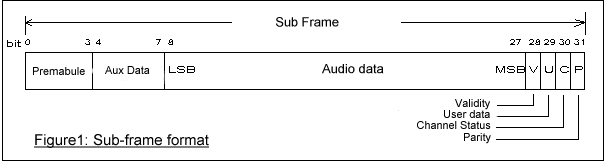
\includegraphics[width=14cm]{_fig1.png}\newline \newline
\noindent
Der Timing Generator verfügt über die folgenden 1 Bit Ein- und Ausgänge: \newline \newline
Eingänge:
\begin{itemize}
\item {\bf CLK:} Taktsignaleingang, dessen Frequenz die verdoppelte Frequenz der eigentlichen Bitrate ist (bei 44kHz Samplerate wird es auf 5.6MHz getaktet).
\end {itemize}
\noindent
Ausgänge:
\begin {itemize}
\item {\bf SHIFTCLK:} legt fest, ob der Shiftregister des Data-Multiplexers die eingehende Daten verschieben soll.
\item {\bf LOAD\_R\textbackslash LOAD\_R:} legt fest, ob die Daten des linken oder rechten Kanals mit Hilfe des Data-Multiplexers an den Biphase-Mark Encoder weitergeleitet werden sollen.
\item {\bf START:} legt fest, ob der Subcode Generator die User Data und Channel Status Bits ausgeben soll.
\item {\bf X\textbackslash Y:} legt fest, ob der Biphase-Mark Encoder eine Präambel für den linken (X) bzw. rechten (Y) Kanal kodieren und ausgeben soll.
\item {\bf Z:} legt fest, ob der Biphase-Mark Encoder eine Präambel für den Anfang eines Blocks kodieren und ausgeben soll.
\item {\bf P:} legt fest, ob der Biphase-Mark Encoder ein Parity-Bit ausgegeben soll.
\end{itemize}
\newpage

\section{Ist-Analyse}

Zur Entwicklung stehen uns folgende Hilfsmittel zur Verfügung:	
\begin{itemize}
\item Vorlesungsunterlagen der ERA-Vorlesung von Prof. Dr. Arndt Bode aus dem WS 12/13
\item GHDL
\item GTKwave
\end{itemize}	

\section{Zeitplan}

\begin{center}
  \begin{tabular}{|*{5}{c|}}
    \hline
	Aufgabe & Jonathan & Arseniy & Amar & Deadline \\
    \hline
   	\multicolumn{1}{|l|}{Pflichtenheft} & 2h & 2h & 2h & 19.05.2013 \\
    \hline
    \multicolumn{1}{|l|}{Spezifikation} & 3h & 3h & 3h & 09.06.2013 \\
    \hline
    \multicolumn{1}{|l|}{Implementierung} & 12h & 12h & 12h & 30.06.2013 \\
    \hline
    \multicolumn{1}{|l|}{Ausarbeitung} & - & 3h & - & 14.07.2013 \\
    \hline
    \multicolumn{1}{|l|}{Vortrag} & 2h & - & 3h & TBA \\
    \hline
    \multicolumn{1}{|l|}{Protokoll} & 3h & - & - &  \\
    \hline
    \multicolumn{1}{|l|}{Summe} & 22h & 20h & 20h &  \\
    \hline
    
    
  \end{tabular}
\end{center}

\section{Vertragsverpflichtung}

Folgende Dokumente sollen im Verlauf des Praktikums abgegeben werden:
\begin{itemize}
\item Protokolle der jeweiligen Sitzungen
\item Pflichtenheft
\item Spezifikation
\item Dokumentation
\item Implementierung des Programms 
\end{itemize}



\end{document}